\documentclass[12pt]{article}
\usepackage[normalem]{ulem}
\usepackage{graphicx, multirow}
\usepackage{amsmath, array}
\usepackage{fancyheadings, lastpage}
\usepackage{pdflscape ,anyfontsize}
\usepackage{longtable}
\usepackage{listings}
\usepackage{algpseudocode}
\usepackage{changepage}
\usepackage[a4paper]{geometry}
\renewcommand{\refname}{}
% REFERENCE http://tex.stackexchange.com/questions/4891/how-do-i-control-the-spacing-above-a-new-paragraph %
\makeatletter
\renewcommand{\paragraph}{
  \@startsection{paragraph}{4}
  {\z@}{3.25ex \@plus -10em \@minus 1em}{0.1em}
  {\normalfont\normalsize\bfseries}
}
\lstset{
    breaklines=true,
  }
\makeatother
\newcommand{\zeroindent}{\setlength{\parindent}{0pt}}
\setcounter{secnumdepth}{5}
\setcounter{tocdepth}{6}
\renewcommand{\headrulewidth}{0pt}
\lhead{Group Project 07 – Design Specification}
\rhead{(Release) -Version 2.9}
\lfoot{Aberystwyth University / Computer Science}
\cfoot{}
\rfoot{\thepage{}  of  \pageref{LastPage}}
\usepackage{graphicx}
\begin{document}
\pagestyle{fancy}
\begin{flushleft}
\rule[0.5cm]{13.8cm}{0.02cm}
\end{flushleft}
{\fontsize{20}{20}\selectfont \textbf {\centerline{Group Project 07 Design Specification}}}
\begin{flushleft}
\rule[0.5cm]{13.8cm}{0.01cm}
\end{flushleft}

\begin{tabular}{ l l }

\\ \multirow{1}{*}{\textit{Authors: }} & Mosopefoluwa David Adejumo \\  & Ryan Gouldsmith \\
& Harry Flynn Buckley \\ & Zack Lott \\ & Mark Radcliffe Pitman \\ & Jack Alexander Reeve \\ & Mark Alexander Smith \\ &Martin Vasilev Zokov \\ & Maciej Wojciech Dobrzanski \\
\\ \multirow{1}{*}{\textit{Config ref: }} & SE\_07\_PM\_01 \\
\\ \multirow{1}{*}{\textit{Date} } & \today \\
\\ \multirow{1}{*}{\textit{Version}} & 2.9 \\ 
\\ \multirow{1}{*}{\textit{Status}} & Release \\

\end{tabular}


\vspace{3.2cm}
\hfill\begin{minipage}{\dimexpr\textwidth-0.3cm}
Department of Computer Science \\
Aberystwyth University \\
Aberystwyth \\
Ceredigion\\
SY23 3DB \\
Copyright \small{\copyright}\\ Aberystwyth University 2013
\end{minipage}


\newpage
\tableofcontents{}
\newpage
\section{INTRODUCTION}
\subsection{Purpose}
The purpose of this document is to, specify the technical design of both the Android and web applications. It will go into detail regarding functions. This will allow us to more easily designate tasks to team members when it comes to coding week. It will also show how these functions interact with each other and how the website, server and Android app interact through the use of sequence diagrams. The document is structured in a way that makes it easy to refer to when the programmer needs clarification on how to build a certain function. The document will also show how the database will be structured and what the field names will be.
\subsection{Scope}
This document, will cover all aspects of the Android and web design and their implementation. It should be read by all members of the group and approved by the client. It will be used as a guide for the programmers to build from in coding week. The document will allow the team leader to assign a given function to a team member which they can then code.
\subsection{Objective}
The precise areas which this document will cover are:
\begin{itemize}
\item Provide a clear class diagram, covering all aspects of the Android app.
\item Define, in detail, the interaction between all the programs in the system.
\item Provide a structure for implementation of the applications.
\item Outline the significant systems to be used in the applications.
\item Provide descriptions of functions.
\end{itemize}
\newpage
\section{ARCHITECTUAL DESCRIPTION}
\subsection{Programs In System}
The walk tour application consists of:
\begin{itemize}
\item The Android application. 
\item The Data server. 
\item The Website application.
\end{itemize}
\subsubsection{The Android Application}
\par{The Android application is used to create physical data representing a route allowing the users to record and upload a walk. It allows the user to add points of interest along a route and associate points of images. It displays a map screen and is used to record location data for a walk using GPS. It also gives the user options to add pictures to a walk. \newline Requirements Covered: (FR1, FR2, FR3, FR4, FR5, FR6, FR7,FR9, EIR1, PR1)}
\subsubsection{The Database Server}
Stores walk info in MySQL which it receives from the Android application as a MIME type. When the server application receives information for a walk it appends the location data to the database and stores all pictures on the server machine. The database server will also have a PHP file which handles the uploading of data from the Android device. The file that handles the upload can be accessed via the URL in a browser, but doing so will present an error message.
Requirements Covered: (DC3)
\begin{itemize}
	\item List of Walks relation:
	\begin{itemize}
		\item id
		\item title
		\item shortDesc
		\item longDesc
		\item hours
		\item distance
	\end {itemize}
	\item Location
	\begin{itemize}
		\item id
		\item walkID
		\item latitude
		\item longitude
		\item timestamp
	\end{itemize}
	\item Place description
	\begin{itemize}
		\item id
		\item locationId
		\item name
		\item description
	\end{itemize}
	\item Photo Usage
	\begin{itemize}
		\item id
		\item placeId
		\item photoName
	\end{itemize}
\end{itemize}
\subsubsection{Web Application}
Allows the user to view walks in more detail. The website is also hosted on the data server and can be used for viewing information about walks including route taken, points of interest and pictures. This program overlaps with 1.1.2 (Database Server). It interacts with the database using PHP. 
Requirements covered: (FR8, FR9)
\subsection{Significant Classes}
\subsubsection{Android Application}
This section describes the most significant classes in the application. The complete set of classes can be seen in the class diagram – Section 4.1.2. These classes will all be written in Java.
\paragraph{WalkModel}
\zeroindent
A WalkModel holds all the data concerning a single route, this includes a list of all location points that trace the path and a list of all the places of interest.
\paragraph{RouteRecorder}
\zeroindent
The RouteRecorder retrieves the current location from the system, and depending on factors such as speed and direction, the location information will be added to the local WalkModel. This class will carry out some analysis of the path traveled so far to determine when to record points,i.e. if a recorded path seems to be traveling in a straight line then fewer point will be need added than if the path traces a circle.
\paragraph{FileTransferManager}
\zeroindent 
A connection will be made with the server via the FileTransferManager. It is responsible uploading and downloading WalkModels, including all associated images, from the database server. This class only interacts with the WalkManager, so any objects wishing to upload of download content must connect through WalkManager, this is to add an extra layer of abstraction that simplifies the solution.
\paragraph{GeneralActivity}
\zeroindent
GeneralActivity is an abstract class that extends Activity. It defines the general layout of all the screens (MainMenuSreen, MapScreen, etc.). It provides subclasses with access to several static variable that describe the layout that allow changes such things as the background, and text colour. All the screens displayed to the user are subclasses of GeneralActivity.
\subsubsection{Database Server}
The files here are used to control the interaction between the database and the other programs in the module. All these files will be written in PHP. Object Oriented Programming will not be implemented in this system.
\subsubsection{Web Application}
The following are files in PHP that will be used to interact between the database and the website. These are also pages that will be visible and accessible by the user unless otherwise stated. Object Oriented Programming will not be implemented in this system.
\paragraph{Index}
This file will serve as the homepage and holds links to view the list of walks and terms of service.
\paragraph{Walk List}
This file will process information from our database and display it as a list of walks.
The walks will be clickable in order to view them in more detail. Users will be able to select a walk via this file
\paragraph{Walk Details}
This file will be used to give the user a more in depth look at a specific walk.
This means they will be able to see a map view, images taken on the walk, and points of interest.
\paragraph{Google Maps Api}
The Google Maps API will be used to portray a persons walk data into a visual map.
The user will also be able to view points of interest on the map. This will serve as a separate file that will interact with Google’s system.
\paragraph{File\_Saver}
The Apache HTTP Client will be used for by the android application to send data to our database server. This will mean our application will be able to 'POST' data to the server. This reduces load on the server compared to our previous idea of zipping and unzipping each set of files for a walk. The data will be sent as a JSON string. This file will decode the JSON string and add all the walk data to the appropriate tables where required
\subsection{Table Mapping Requirements Onto Classes}
This section gives an overview of what classes/files cover what requirements as specified by the client.

\begin{tabular}{|p{1cm}|p{10cm}|}
\hline
	FR1 & GeneralActivity, MapScreen, WalkSetupScreen, MyWalksScreen, MainMenuScreen, OptionsScreen, WalkInfoView\\
\hline
	FR2 & MapScreen, RouteRecorder, WalkModel\\
\hline
	FR3 & LocationPoint, PointOfInterest\\
\hline
	FR4 & LocationPoint, PointOfInterest\\
\hline
	FR5 & WalkInfoView\\
\hline
	FR6 & WalkManager, FileTransferManager
\\
\hline
	FR7 & RouteRecorder\\
\hline
\end{tabular}
\newpage
\section{DEPENDENCY DESCRIPTIONS}
\subsection{Component Diagrams}
\subsubsection{Android}
\begin{figure}[htp]
\centering
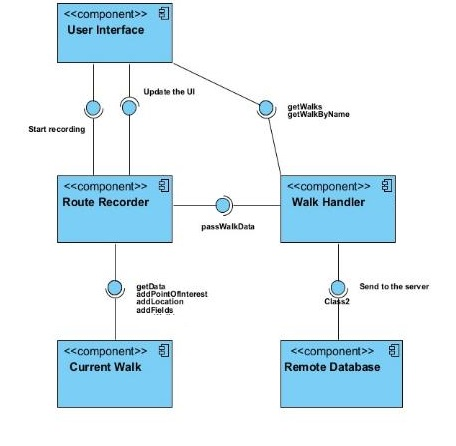
\includegraphics[scale=0.90]{Design/AndroidDP.jpg}
\caption{Android Dependency Diagram}
\label{Android Dependency Diagram}
\end{figure}

\subsubsection{Website}
\clearpage
\begin{figure}[htp]

\centering
\includegraphics[scale=0.50]{Design/web_diagram.png}
\caption{Web Component Diagram}
\label{Web Component Diagram}
\end{figure}
\subsubsection{Database Server}
\section{INTERFACE DESCRIPTION}
This section contains an implementation of different classes and files in the program. However, there is a possibility that the implementation in the final product may differ from what is displayed here.
\subsection{Screens}
The following classes all extend Activity and are used to control the display.
\subsubsection{OptionsScreen}
\begin{lstlisting}[language=java]
public class OptionsScreen extends GeneralActivity {
	/**
	 * This method changes the background color,
	 * of all generalActivity subclasses
	 * @param v, is the object that called the method.
	 */
	public void changeBackgroundColor(View v);
}
\end{lstlisting}
\subsubsection{MainMenuScreen}
\begin{lstlisting}[language=java]
public class MainMenu extends GeneralActivity {

	/**
	 * Starts a new MyWalkScreen activity,
	 * and displays it to the user.
	 *@param v, is the object that called the method.
	 */
	public void startMyWalksScreen(View v);

	/**
	 * Starts a new WalkSetupScreen activity,
	 * and displays it to the user.
	 * @param v, is the object that called the method.
	 */
	public void startWalkSetupScreen(View v);
	
	/**
	 * Starts a new OptionsScreen activity,
	 * and displays it to the user.
	 * @param v, is the object that called the method.
	 */
	public void startOptionsScreen(View v);

	/**
	 * Starts a new LoginScreen activity,
	 * and displays it to the user.
	 * @param v, is the object that called the method.
	 */
	public void StartLoginScreen(View v);
}
\end{lstlisting}
\subsubsection{MyWalkScreen}
\begin{lstlisting}[language=java]
public class MyWalksScreen extends GeneralActivity {
	
	/**
	 * open a WalkInfoView popup on selected walk
	 * @param v, is the object that called the method.
	 */
	public void viewWalk(View v);
}
\end{lstlisting}
\subsubsection{WalkSetupScreen}
\begin{lstlisting}[language=java]
public class WalkSetupScreen extends GeneralActivity {
	
	/**
	 * Starts a new MapScreen activity
	 * and displays it to the user.
	 * The detail that the user has input,
	 * are passed to the new activity.
	 * @param v, is the object that called the method.		
	 */
	public void startWalk(View v);
}
\end{lstlisting}
\subsubsection{MapScreen}
\begin{lstlisting}[language=java]
public class MapScreen extends GeneralActivity {
	
	/**
	 * creates and displays a AddPoiView.
	 * @param v, is the object that called the method.
	 */
	public void addPOI(View v);
	
	/**
	 * creates and displays a WalkFinishedView.
	 * @param v, is the object that called the method.
	 */
	public void finishWalk(View v);
	
	/**
	 * creates and displays a PlacesVisitedView.
	 * @param v, is the object that called the method.
	 */
	public void showPlacesVisited(View v);

}
\end{lstlisting}
\subsubsection{GeneralActivity}
\begin{lstlisting}[language=java]
public abstract class GeneralActivity extends Activity{

	/**
	 * changes the background color of all GeneralActivity
	 * subclasses to the passed
	 * value. The int c, represents a color.	
	 */
	public void setBackgroundColor(int c);

	/**
	 * changes the foreground color of all
	 * GeneralActivity subclasses to the passed 
	 * value. The int c, represents a color.	 		
	*/
	public void setForegroundColor(int c);

	
	/**
	 * changes the text color of all GeneralActivity
	 * subclasses to the passed value.
	 * The int c, represents a color.
	 */
	public void setTextColor(int c);
}
\end{lstlisting}
\subsection{Views}
\subsubsection{MapView}
\begin{lstlisting}[language=java]
public class MapView/*our class*/ extends MapFragment/*from google API*/{
	/**
	 * sets the walks that is to be displayed
	 */	
	public void setWalk(WalkModel walk);
		
	/**
	 * this method will cause the map 'window' 
	 *	to redraw the route on to itself.
	 */
	public void updateWalk();
}
\end{lstlisting}
\subsubsection{WalkInfoView}
\begin{lstlisting}[language=java]
public class WalkInfoView extends PopupView{

	/**
	 * creates a WalkInfoView instance.
	 * The WalkModel that is passed to it 
	 *is displayed in in the popup.  
	 */
	public class WalkInfoView(WalkModel walk);
}
\end{lstlisting}
\subsubsection{PopupView}
\begin{lstlisting}[language=java]
public abstract class PopupView extends DialogFragment {
	/**
	 * closes the popup view.
	 * @param v, is the object that called the method.
	 */
	public void closePopup(View v);
}
\end{lstlisting}
\subsubsection{PoiInfoView}
\begin{lstlisting}[language=java]
public class PoiInfoView extends PopupView{		
			
	/**
	 * creates a PoiInfoView instance. The PointOfInterest
	 * that is passed to it
	 *is displayed in in the popup.  
	 */
	public void PoiInfoView(PointOfInterest point);
}
\end{lstlisting}
\subsubsection{PlacesVisitedView}
\begin{lstlisting}[language=java]
public class PlacesVisitedView extends PopupView{
	/**
	 * creates a PlacesVisitedView instance.
	 * All the PointOfInterest from the 	
	 *passed walk are displayed in a table.
	 */
	public void PlacesVisitedView(WalkModel walk);		

	/**
	 * opens a PoiInfoView.
	 * @param v, is the object that called the method.
	 */
	public void getPoiInfo(View v);
}
\end{lstlisting}
\subsubsection{WalkFinishedView}
\begin{lstlisting}[language=java]
public class WalkFinishedView extends PopupView{
	/**
	 * displays a screen displaying
	 * a summary of the finished walk, and 
	 * shows various options to the user regarding the WalkModel.
	 */
	public void WalkFinishedView(WalkModel walk);

	/**
	 * open a PoiInfoView
	 * @param v, is the object that called the method.
	 */
	public void uploadWalk(View v);
}
\end{lstlisting}
\subsubsection{AddPoiView}
\begin{lstlisting}[language=java]
public class AddPoiView extends PopupView{
	/**
	 * displays an place description input popup,
	 *  and gives it a link to the RouteRecorder
	 */
	public void AddPoiView(RouteRecorder recorder);

	/**
	 * creates a PointOfInterst out of the given
	 * data (from text fields) and 	add the point the the WalkModel
	 * @param v, is the object that called the method.	
	 */
	public void submit(View v);
	
	/**
	 * uses ImageHandler to open the photoLibrary,
	 * the selected photo is then added to the PointOfInterest.
	 * @param v, is the object that called the method.
	*/
	public void getPhotoFromLibrary(View v);

	/**
	 * uses ImageHandler to open the camera app,
	 * the taken photo is then added to the PointOfInterest.
	 * @param v, is the object that called the method.
	 */
	public void getPhotoFromCamera(View v);
}
\end{lstlisting}
\subsection{Models}
\subsubsection{WalkModel}
\begin{lstlisting}[language=java]
public class WalkModel {	

	/**
	 * creates a WalkModel, with LocationPoints already set, it is used 
	 *by the WalkManager when loading walk from database.
	 */
	public WalkModel(String title,Vector<LocationPoint> path,String shortDesc,String longDesc);

	/**
	 * @return a vector of all the LocationPoint in the walk.
	 */
	public Vector<LocationPoint> getRoutePath();
	
	/**
	 * @return the running total of km travelled.
	*/
	public double getDistance();
	
	/**
	 * @return the elapsed time since the walk was started.
	 */
	public double getTimeTaken();
	
	/**
	 * @return the name of the walk.
	 */
	public String getTitle();
	
	/**
	 * @return a short description of the walk
	 */	
	public String getShortDescription();
	
	/**
	 * set the short description of the walk.
	 */
	public void setShortDescription(String newShortDesc);
		
	/**
	 * @return a long description of the walk.
	 */
	public String getLongDescription();
	
	/**
	 * set the long description for the walk.
	 */
	public void setLongDescription(String newLongDesc);
	
	/**
	 * adds a LocationPoint to the walk.
	 */
	public void addLocation(LocationPoint point);
}
\end{lstlisting}
\subsubsection{LocationPoint}
\begin{lstlisting}[language=java]
public class LocationPoint {

	/**
	 * creates a new LocationPoint
	 */
	public LocationPoint(double x,double y);
	
	/**
	 * creates a LocationPoint,
	 *  used to recreate a point stored in the
	 *database.
	 */
	public LocationPoint(double x,double y,double time);
	
	/**
	 * @return the time at which the point was recorded.
	 */
	public double getTime();
		
	/**
	 * @return the longitude, the east/west
	 * distance from Greenwich. 
	 */
	public double getLongitude();
		
	/**
	 * @return the latitude, the north/south distance from the equator.
	 */
	public double getLatitude();
	
	/**
	 * @return the distance between itself and a passed point.
	 */
	protected double distanceTo(LocationPoint point);
}
\end{lstlisting}
\subsubsection{PointOfInterest}
\begin{lstlisting}[language=java]
public class PointOfInterest extends LocationPoint{

	/**
	 * creates a PointOfInterest, at position x,y.
	 *  The time is set automatically
	 */
	public PointOfInterest(double x,double y);
	
	/**
	 * creates a PointOfInterest, at position x,y.
	 * The time is also explicitly defined, this is 
	 * used when creating a PointOfInterest from a database entry.
	 */
	public PointOfInterest(double x,double y,double time);
	
	/**
	 * @return all the images associated with this point.
	 */
	public Vector<ImageInformation> getImages();

	/**
	 * @return the description of this place.
	 */
	public String getDescription();

	/**
	 * sets the description of this point.
	 */
	public void setDescription(String desc);
}
\end{lstlisting}
\subsection{Controllers}
\subsubsection{RouteRecorder}
\begin{lstlisting}[language=java]
public class RouteRecorder extends Service implements LocationListener{
		
	/**
	 * creates a RouteRecorder instance,
	 *  with the MapView that will display the walk.
	 */
	public RouteRecorder(MapView map);
	
	/**
	 * starts the recording of location points
	 */
	public void startRecording();
	
	/**
	 * adds a PointOfInterest to the recorded path.
	 */
	public void savePoi(PointOfInterest poi);
	
	/**
	 * stops the recoding of locations.
	 */
	public void finish();
}
\end{lstlisting}
\subsubsection{FileTransferManager}
\begin{lstlisting}[language=java]
public class FileTransferManager{
		
	/**
	 *@param walk 
	 * makes a connection to data server and
	 *  uploads all files belonging to the given
	 * file, the return values will be zero if
	 *  the method succeeded without problems.		
	 */
	public int uploadWalk(WalkModel walk);
}
\end{lstlisting}
\section{DETAILED DESIGN}
This section details the algorithms and interactions that will be implemented in the program. The algorithms used may differ from the final product.
\subsection{UML Diagrams}
\subsubsection{Android Sequence Diagram}\clearpage
\begin{figure}[htp]

\begin{adjustwidth}{-3cm}{0cm}
\centering
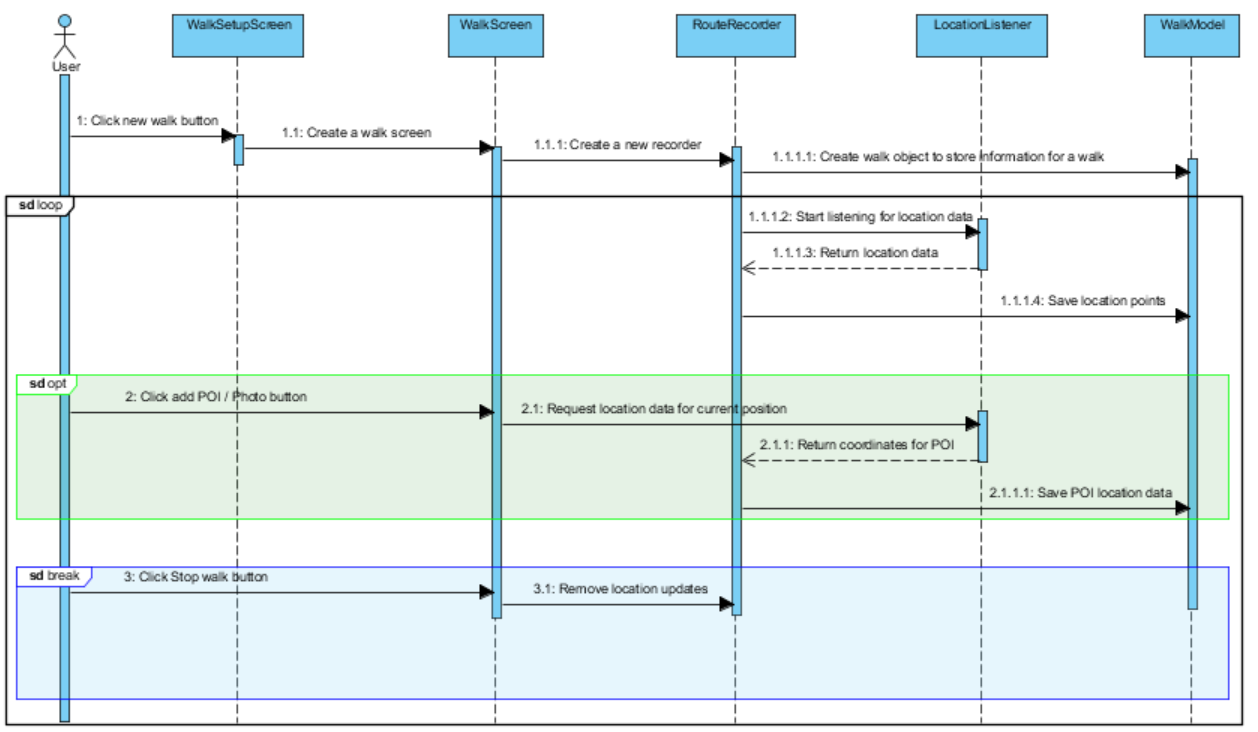
\includegraphics[scale=0.90]{Design/route_record_sequence_diagram.PNG}
\caption{Android Sequence Diagram}
\label{Android Sequence Diagram}
\end{adjustwidth}
\end{figure}
The sequence diagram describes the recording of a walk and how the classes which are involved in the process interact.
In action 1. the user is prompted for details in the WalkSetupScreen and after he/she presses the start walk button, a map screen is shown and a RouteRecorder and WalkModel objects are created. After that the application goes into a loop of actions from the RouteRecorder, LocationListener and WalkModel classes. The recorder asks the listener for location data and when the data is returned, it is saved in the WalkModel's array of location points.
Action 2 is optional for the user, because it is not mandatory to have a Point of interest or photos in every walk. If a user decides to click the “Add POI” button, the LocationListener gives the coordinates of the current location to the RouteRecorder and they are saved in the WalkModel object.
Action 3 is the exit point of the loop for the current walk recording. It is done by clicking the stop button which brakes the loop and saves the last set of coordinates for the current walk.
The LocationListener is deliberately not activated at all times while a walk is in progress in order to save battery life.
\subsubsection{Sequence Diagram For Web}
\begin{figure}[htp]
\begin{adjustwidth}{-2cm}{0cm}
\centering
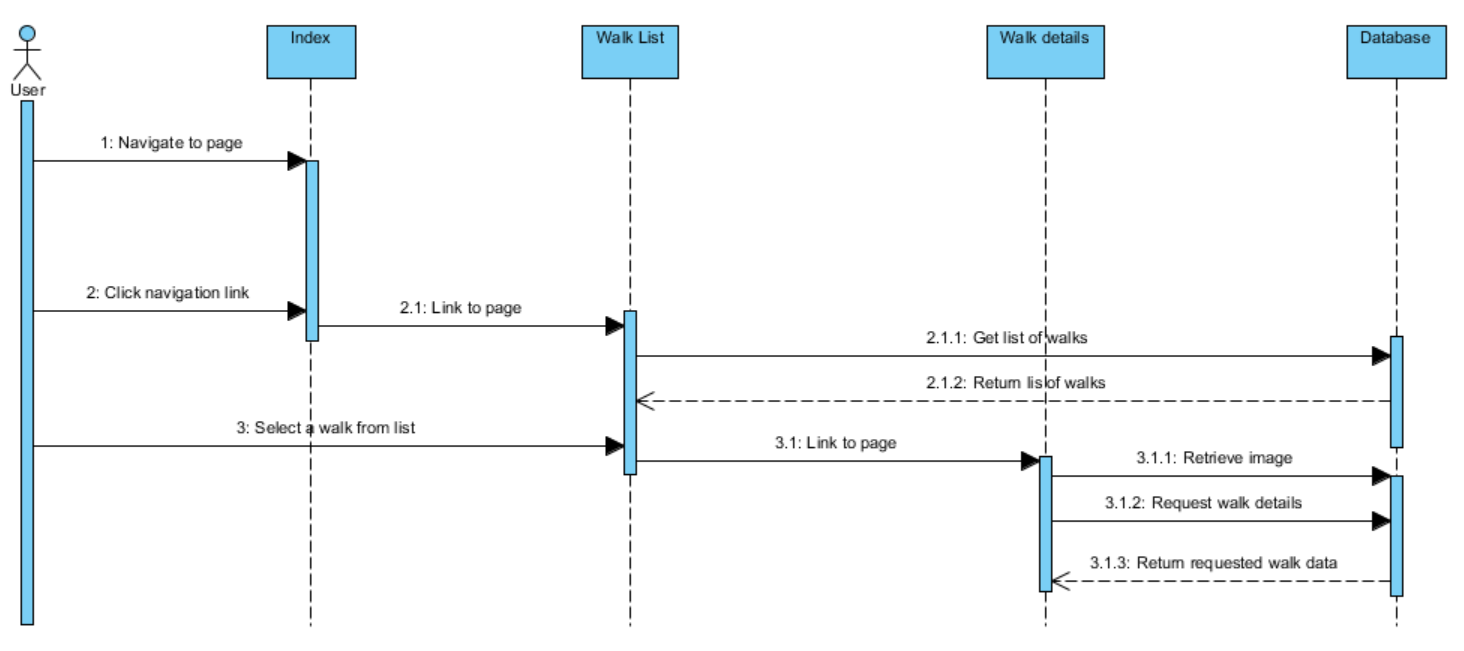
\includegraphics[scale=0.70]{Design/web_sequence_diagram.PNG}
\caption{Web Sequence Diagram}
\label{Web Sequence Diagram}
\end{adjustwidth}
\end{figure}
\subsubsection{Overall Interaction Sequence Diagram}

\subsection{Class Diagram}
\newgeometry{top=1.5cm, bottom =-0.8cm}
\begin{landscape}
\begin{adjustwidth}{0.5cm}{2cm}
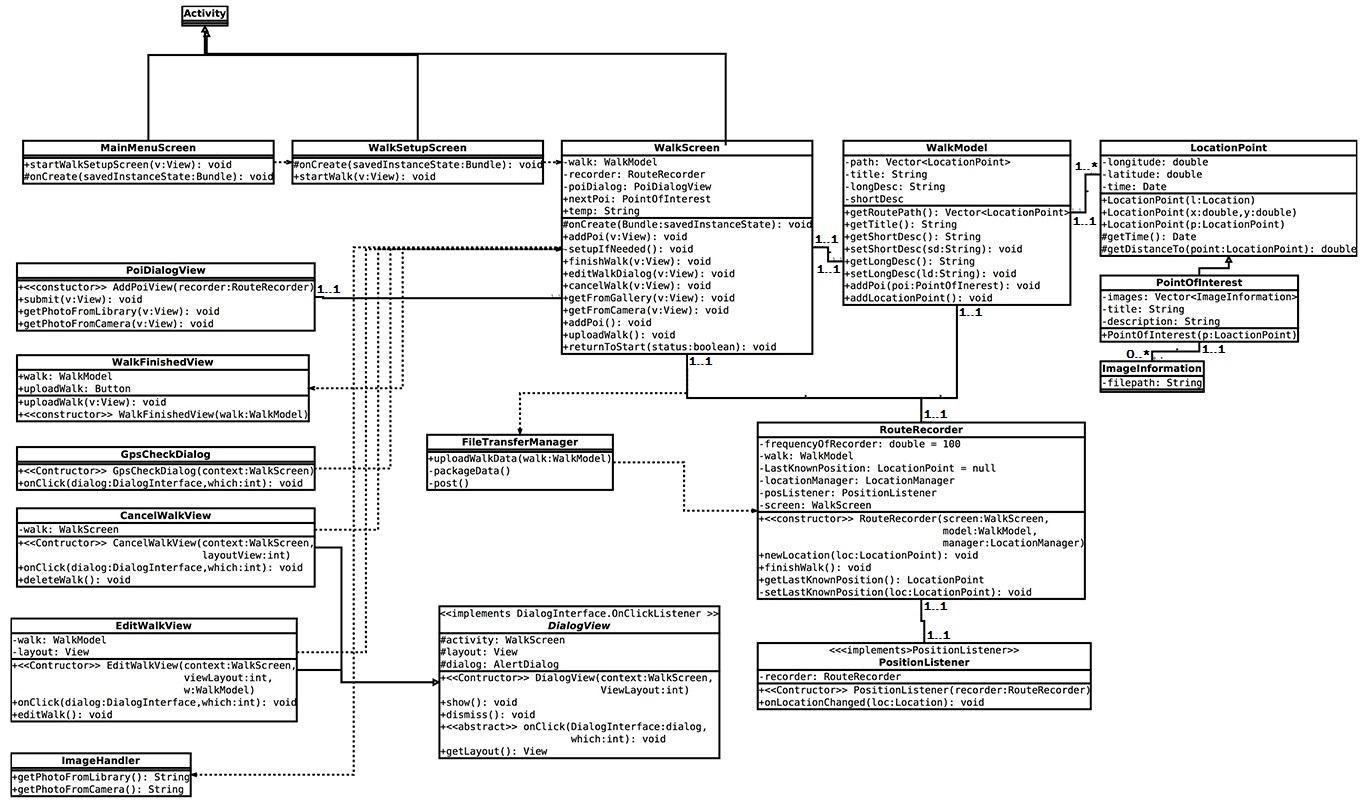
\includegraphics[scale=2.74253]{Design/class_diagram_new.jpg}
\end{adjustwidth}
\end{landscape}
\restoregeometry
The classes ending in ‘screen’, are all Activities. They all, in some way, display a layout to the screen and respond to user input. Any response that requires further processing would be passed to another class and then handed back to be displayed, but it would be the ’screen’ class itself that initialised the action.  
There are several classes that have been suffixed with ‘View’, these classes all extend the android class View. They are all visible to the user and act much like ‘screen’ classes except that they don’t use the whole screen and do not change the displayed screen only create new Views.  
The classes WalkModel,PointOfInterest and Location can all be considered to be model classes. There are used to store the walks data in an organised fashion, and have no methods to do anything other than to set and get information.  
WalkManager, ImageHandler and FileTransferManager all perform some tasks that are not immediately apparent the user. They are the utility classes that are used by others.
\subsection{Significant Algorithms}
\subsubsection{Android Algorithms}
\paragraph{RouteRecorder Algorithm}
\zeroindent
\begin{algorithmic}
\While{walk not finished}
	\State get location
	\If{distance between new location, old location than X}
		\State add new location to walkModel
	\EndIf
\EndWhile
\end{algorithmic}
\subsubsection{PHP Algorithms}
\paragraph{Connect To The Database}
\zeroindent
\begin{lstlisting}
/**
* This is the function to connect to the a database
*/ 
connectToDatabase();


/**
* This code will connect to our own database with our database name,
* username and password
*/  
$con=mysqli_connect("db.dcs.aber.ac.uk”, “csgp07_13_14”,"csadmgp07","c54admgp07");

/*
* If the php fails to connect to the database this will appear
*/
//heck connection
if(mysqli_connect_errno())
{
	echo "Failed to connect to MySQL: " . mysqli_connect_error();
}
mysqli_close($con);
\end{lstlisting}
\paragraph{Append To The Server Database}
\begin{adjustwidth}{-3cm}{-3cm}
\begin{lstlisting}
$sql = "INSERT INTO List_of_Walks(title, shortDesc, longDesc, hours, distance) VALUES('$title','$short_desc', '$long_desc', '$hours', '$distance')"; 

mysqli_query($walk_conn,$sql);
    
$walkID = mysqli_insert_id($walk_conn);	
		
foreach($route as $loc){
       
			
	$longitude = $loc['longitude'];           
	$latitude = $loc['latitude'];            
	$time = $loc['time'];			
	$sql = "INSERT INTO Location(walkID, latitude, longitude, timestamp)VALUES('$walkID','$latitude','$longitude', '$time')";
            
	mysqli_query($walk_conn,$sql);
        
	$locID = mysqli_insert_id($walk_conn);
	if(isSet($loc['description'])){			
		$description = $loc['description'];
		$name = $loc['title'];
		$sql = "INSERT INTO Place_description(description, locationId, name)values('$description', '$locID', '$name')";
		mysqli_query($walk_conn,$sql);
		$placeId = mysqli_insert_id($walk_conn);
			if(isSet($loc['images']))\{
				$photoCount = 0;
				foreach($loc['images']as $image)\{
				
					$image = implode($image);
						
					$image =  base64_decode($image);
						
					$photoName = $walkID . "_" . $locID . "_" . $placeId . "_" . $photoCount;
						
					file_put_contents("images/".$photoName . ".jpg",$image);
						
					$photoCount++;
						
					$sql = "INSERT INTO Photo(photoName, placeId)values('$photoName', '$placeId')";
						
					mysqli_query($walk_conn,$sql);
						
					}
					
				}
				
			}
\end{lstlisting}
\end{adjustwidth}
\subsection{TODO CHECK THE ALGORITHMS}
\subsection{Significant Data Structures}
\subsubsection{WalkModel}
This is the most significant data structure in the Android application. It contains the infor-
mation for the route taken,
all of the GPS coordinates that the user has walked through, Points of interest.
\subsubsection{LocationPoint}
This class is responsible for storing a point on the map. It has variables for longitude, lati-
tude and a timestamp.
After a GPS reading is taken for the current physical location is taken, it is put in an object
of this class and stored in the WalkModel.
\subsubsection{PointOfInterest}
This data structure is used when adding a point of interest. It holds information for the de-
scription and title of a POI.
The class extends the LocationPoint so a POI can have location coordinates and a time
stamp.
This data structure is used when adding a point of interest. It holds information for the de-
scription and title of a POI.
The class extends the LocationPoint so a POI can have location coordinates and a time
stamp.
\newpage 
\section{REFERENCES}
\begin{thebibliography}{0}
\bibitem{Requirements1.2}
  Software Enginerring Group Projects
  \emph{Requirements Specification}.
   C. J. Price and B.P.Tiddeman, 
   1.2 (Release), 
   7 November 2013
\bibitem{DesignStand 1.6}
Software Engineering Group Projects. 
\emph{Design Specification Standards}.
	C. J. Price and N. W. Hardy, 
	SE.QA.05A,
	1.6. Release.
\bibitem{ProjectPlan1.8}
Software Engineering Group Projects
\emph{ Project Plan}.
Mosopefoluwa David Adejumo -all names-, 1.8
(Release). 6th November 2013
\end{thebibliography}
\newpage

\section{DOCUMENT HISTORY}
\setlength\LTleft{-0.5cm}
\begin{longtable}{|p{1.3cm}|p{1.5cm}|p{2cm}|p{7cm}| p{2cm}|}
\hline
	Version & CFF No. & Date & Section Changed From Previous Version & Changed by \\
\hline
	1.0 & N/A & 28/11/13 & Created original document & HFB1 \\ 
\hline
	1.1 & N/A & 01/12/13 & Added sections created by other members. 
Updated config reference 
Updated layout. & MDA
 \\
\hline
	1.2 & N/A & 01/12/13 & Fixed some formatting issues, added information to what fields will be used. & RYG1 \\
\hline 
	1.3 & N/A & 04/12/13 & Added a new sequence diagram and a description for section 1.2 & MVZ
\\
\hline 
	1.4 & N/A & 05/12/13 & Updated section 1.1. Added descriptions to all sections & MDA \\
\hline 
	1.5 & N/A & 05/12/13 & Added a sequence diagram for the web.
 & MRP2 \\
\hline
	1.6 & N/A & 05/12/13 & Updated class diagram, added FileTransferManager interface. & HFB1 \\
\hline 
	1.7 & N/A & 06/12/13 & Added Apache HTTP Client description. & JAR39 \\
\hline 
	1.8 & N/A & 06/12/13 & Added methods to the MapView interface. & HFB1
 \\
\hline	
	1.9 &N/A&06/12/13&Changed sequence diagram for web and added
overall interaction sequence diagram & MVZ\\
\hline 
	2.0&N/A&06/12/13&Updated the Introduction section.&JAR39,
MRP2 \\
\hline
	2.1&N/A&06/12/13&Added web app diagram and Significant algorithms &ZAL \\
\hline 
	2.2&N/A&06/12/13&Updated author list. Updated formatting. Merged different versions of the document&MDA\\
\hline
	2.3&N/A&06/12/13& Added image reference numbers. Updated images 
from MWD5 and MAS69. Added missing images. Added images and descriptions to section 3.Added references. & MDA\\
\hline 
	2.4&N/A&06/12/13&Formatting corrections. Changed version&MDA \\
\hline 
	2.5&N/A&12/02/14&Re-wrote in LaTeX, removing feature creep &RYG1 \\
\hline
	2.6&N/A&13/02/14&Minor error checks and removal &MDA \\
 \hline
 	2.7&N/A&13/02/14&Added Images & RYG1\\
 \hline
 2.8&N/A&13/02/14&Added Sequence Diagrams &RYG1\\
 \hline
 \hline
 2.9&N/A&13/02/14&Updated database file saver algorithm &MDA\\
 \hline
\end{longtable}


\end{document}